% =====================================================================================
%  Economic evaluation: LP vault backtest and tail-decision value
%  Insert blocks for manuscript.tex (cas-sc class, natbib authoryear).
%  Each block below says where it goes. New references: economic_evaluation_refs.bib
%  (append to updated.bib). Figures: copy ./figures/*.pdf into the manuscript's figures/.
%  Code and outputs: 14. LP vault backtest/ (run_all.py, frontier.py, tail_marginal.py,
%  fc_gate.py, compounding.py).
%  Units: bp = basis points of vault capital; "net" = PnL against a delta-matched
%  rebalancing portfolio (fees + LVR - costs).
% =====================================================================================


% -------------------------------------------------------------------------------------
% [A] ABSTRACT -- append after the forecasting-results sentence
% -------------------------------------------------------------------------------------
In an economic evaluation on the same pool, liquidity ranges set from the forecaster's
predictive quantiles earn 395 basis points per year net of loss-versus-rebalancing and
costs, 114 basis points more than a volatility-scaled benchmark; the forecaster's tail
probabilities give the best-scored protection decisions among all benchmarks; and
classifier gating cuts the vault's maximum drawdown by 63--83\%, with most of its return cost
recovered when alerts are filtered by the forecaster's expected shortfall.


% -------------------------------------------------------------------------------------
% [B] HIGHLIGHTS -- add one item (cas limit: 85 characters)
% -------------------------------------------------------------------------------------
\item Forecast-driven LP ranges beat a volatility-scaled benchmark by 114 bp a year.


% -------------------------------------------------------------------------------------
% [C] INTRODUCTION -- insert before "The remainder of the paper is organized as follows."
% -------------------------------------------------------------------------------------
Third, we evaluate the framework by the value of the decisions it supports rather than by
statistical scores alone \citep{LeitchTanner1991,GrangerPesaran2000}. Both models drive a
concentrated-liquidity vault on the USDC--USDT pool over the holdout, with profit and loss
measured against a delta-matched rebalancing portfolio, net of loss-versus-rebalancing
\citep{Milionis2022}, gas and swap costs, and with a one-hour execution lag. Ranges set from the
forecaster's quantiles earn significantly more than standard benchmarks, including Gamma-style
recentering and volatility-scaled ranges. Classifier gating reduces drawdowns and daily tail
losses significantly relative to randomly timed alerts with the same budget. In tail-protection
decisions at 10 and 15 basis points, the forecaster's exceedance probabilities obtain the best
log and Brier scores and the highest economic value in more cost-loss settings than any
benchmark, consistent with its threshold-weighted CRPS gains.


% -------------------------------------------------------------------------------------
% [D] METHODOLOGY -- new subsection, after Section "Modeling Approach" (end of Sec. 3)
% -------------------------------------------------------------------------------------
\subsection{Economic evaluation design}\label{sec:econ_design}

Detection rates and scoring rules do not establish that a model is economically useful. We
therefore evaluate both models through a liquidity-provision problem on the pool they monitor.
A liquidity provider (LP) operates a concentrated-liquidity vault in the USDC--USDT 0.01\% pool,
similar to automated vaults that manage Uniswap V3 positions on behalf of depositors. The
vault decides, every hour, the price range in which its capital is deployed. Narrow ranges earn
a larger share of swap fees but must be repositioned more often, which costs gas and swap fees,
and expose the LP to adverse selection by arbitrageurs when the price moves
\citep{Milionis2022}.

\paragraph{Position value and fee income.} Let $P_k$ denote the pool price of USDC in USDT at
the end of hour $k$. A position with liquidity $L$ on the range $[p_a,p_b]$ holds
\begin{equation}
x(P)=L\left(\frac{1}{\sqrt{\bar P}}-\frac{1}{\sqrt{p_b}}\right),\qquad
y(P)=L\left(\sqrt{\bar P}-\sqrt{p_a}\right),
\end{equation}
with $\bar P=\min\{\max\{P,p_a\},p_b\}$,
units of USDC and USDT, with value $V(P)=x(P)P+y(P)$ \citep{uniswap_whitepaper}. Fee income in
hour $k$ is
\begin{equation}
f_k=F_k\,\omega_k\,\frac{L}{L^{\mathrm{act}}_k+L},
\end{equation}
where $F_k$ is the fee revenue of the pool, $L^{\mathrm{act}}_k$ its active liquidity, and
$\omega_k$ the share of the hour's high--low price interval that lies inside $[p_a,p_b]$. The
vault's own liquidity dilutes its fee share.

\paragraph{Loss-versus-rebalancing and net PnL.} Following \citet{Milionis2022}, the LP's
convexity loss in hour $k$ is measured against a portfolio that holds the same USDC inventory at
the start of the hour and rebalances at market prices:
\begin{equation}
\mathrm{LVR}_k=V(P_k)-V(P_{k-1})-x(P_{k-1})\,(P_k-P_{k-1})\le 0 .
\end{equation}
The vault's net profit against this rebalancing portfolio is
\begin{equation}
\Pi_k=f_k+\mathrm{LVR}_k-c_k ,
\end{equation}
where $c_k$ collects gas (\$10 per burn and mint) and the cost of swapping the inventory
imbalance at re-minting (1\,bp pool fee plus 0.5\,bp slippage). Total vault value obeys
$V_T-V_0=\sum_k \Pi_k+\sum_k X_{k-1}(P_k-P_{k-1})$, where $X$ is the vault's total USDC
holding. The second term is the common USDC/USDT price exposure, so $\Pi$ isolates what the
LP's decisions add. We report annualised $\sum_k\Pi_k$ in basis points of a \$1M vault,
fee income and LVR separately, the Sharpe ratio of daily $\Pi$, the Sortino ratio, the
maximum drawdown of cumulative $\Pi$, the worst day, and the number of repositionings per
month. The Sortino ratio divides mean hourly $\Pi$ by its downside deviation
$\sqrt{\overline{\min(\Pi_k,0)^2}}$ and is annualised with $\sqrt{8766}$. We compute it hourly
because the vault's losses are intraday LVR spikes that daily aggregation nets against same-day
fee income. Fees are held as
cash in the base case; reinvesting them is reported as a robustness check.

\paragraph{Strategies.} Standard benchmarks are a static range of $\pm5$ ticks around parity, a
Gamma-style vault that recentres a $\pm w$-tick range whenever the price leaves it, and a
volatility-scaled vault whose half-width equals the trailing 24-hour range of the depeg. The
static width and the volatility scaling are the best choices on June 2023 to December 2024
data, before the holdout; the Gamma-style width of $\pm2$ ticks is the best recentering width
in the holdout itself, which favours this benchmark. The classifier gates the recentering vault: during an alert episode,
defined by the operating cutoff and 12-hour quiet reset of Section~\ref{sec:holdout_results},
the vault does not reposition (``freeze''). The forecaster sets the range width: the
half-width equals half the width of the union of the 10\%--90\% predictive intervals over the
next six hours, centred on the median forecast, and the vault recentres when the price leaves
the range or the target width changes by more than a factor of two. The two-model vault
combines the forecaster's ranges with the classifier's freeze.

\paragraph{Tail-based strategies.} The forecaster's lower and upper expected shortfall,
\begin{equation}
\mathrm{ES}^{-}_{a}=\frac{1}{a}\int_0^{a}q(u)\,du,\qquad
\mathrm{ES}^{+}_{a}=\frac{1}{a}\int_{1-a}^{1}q(u)\,du,
\end{equation}
with $q$ the predictive quantile function, enter three further rules. The ES band sets the asymmetric range
\begin{equation}
\left[\,m-\kappa\,(m-\mathrm{ES}^{-}_{0.05}),\;\; m+\kappa\,(\mathrm{ES}^{+}_{0.05}-m)\,\right]
\end{equation}
around the median $m$ over the next six hours, with $\kappa=0.5$, so the range extends further on
the side where the forecast tail is heavier. The ES-filtered gate keeps a classifier alert only
while the 24-hour expected shortfall on either side lies more than 10\,bp from the current
price, so that alerts in calm conditions do not freeze the vault. The ES-sized vault deploys a
share $\min\{1,\max(0.25,\bar s_k/s_k)\}$ of its capital, where $s_k$ is the 24-hour ES
distance from the median and $\bar s_k$ its trailing 30-day median.

\paragraph{Timing and controls.} Decisions are taken at the end of hour $k$ for hour $k+1$.
Price-based rules react to $P_k$ immediately, whereas model outputs stamped $k$ are used from
the end of hour $k+1$, reflecting a one-hour data lag; forecasts are therefore used from
horizon two onwards. Three controls separate the information in the models from the act of
gating: a price trigger that freezes the vault when $|d_k|\ge 8$\,bp, calibrated to the same
share of alert hours as the classifier (11.8\% against 11.6\%); an oracle that knows each
event 24 hours ahead; and 500 placebo schedules that place the classifier's 43 alert episodes,
with their durations, at random dates. Each benchmark forecaster from
Section~\ref{sec:results} is plugged into the identical width rule. Differences in daily net
PnL are tested with the stationary bootstrap \citep{PolitisRomano1994} with a mean block
length of seven days.

\paragraph{Tail decisions.} To evaluate the tail of the predictive distribution, which the
width rule barely uses, we score each forecaster's exceedance probability
$\hat p_{t,h}=\Pr(|d_{t+h}|\ge c)$ for $c\in\{10,15\}$\,bp and $h\in\{6,12,24\}$ hours with
the log and Brier scores, and with the relative economic value of a cost--loss protection
rule \citep{Richardson2000}. A user who pays a protection cost $C$ to avoid a loss $L$ protects
whenever $\hat p\ge r=C/L$. With $\bar y$ the event frequency, the expense per unit loss is
$E_{\mathrm{f}}=\overline{\mathbb 1\{\hat p\ge r\}\,r+\mathbb 1\{\hat p<r\}\,y}$, and
\begin{equation}
\mathcal V(r)=\frac{\min(r,\bar y)-E_{\mathrm f}}{\min(r,\bar y)-\bar y\,r},
\end{equation}
which equals one for perfect foresight, zero for the best constant policy and is negative
when the forecast is worse than that policy.


% -------------------------------------------------------------------------------------
% [E] RESULTS -- new subsection, after the probabilistic forecasting results (end of Sec. 4)
% -------------------------------------------------------------------------------------
\subsection{Economic evaluation}\label{sec:econ_results}

\subsubsection{Liquidity-provision vault}

Table~\ref{tab:lp_main} reports the vault backtest over the common holdout coverage of both
models, 15 January 2025 to 4 May 2026 (11,367 hours, five eligible events). Ranges set from
our forecaster earn 395\,bp per year net of LVR and costs, compared with 346\,bp for the
Gamma-style vault and 281\,bp for the volatility-scaled vault. The differences are significant
under the stationary bootstrap: $+114$\,bp per year against the volatility-scaled vault (95\%
CI: 73--160) and $+49$\,bp against Gamma-style recentering (23--80). Our forecaster also
outperforms TimeXer ($+38$\,bp, 10--68), GARCH, ARIMA and the naive forecast
(Table~\ref{tab:lp_bootstrap}).

LVR absorbs 18--27\% of gross fees for every active vault, so the binding economic risk for a
stablecoin LP is adverse selection combined with repositioning costs rather than the level of
the depeg. Depeg windows are fee-rich: the five events add 21--85\,bp to every active vault.
Exiting ahead of events is therefore not the relevant protective action; avoiding repositioning
into a transient dislocation is. The oracle earns less than the ungated Gamma-style vault (317
against 346\,bp per year), confirming that knowledge of event timing alone has limited value for
an LP that can react every hour.

\begin{table}[pos=!htbp,align=\centering]
\centering
\caption{Liquidity-provision vault on the USDC--USDT 0.01\% pool, 15 January 2025 to 4 May 2026.
Values are in basis points of a \$1M vault. Net is profit against a delta-matched rebalancing
portfolio: fees plus loss-versus-rebalancing (LVR) minus gas and swap costs. Sharpe is computed
on daily net PnL and the Sortino ratio on hourly net PnL; maximum drawdown and worst day refer
to cumulative and daily net PnL. Model signals are used with a one-hour lag. ``Width'' rows use
the same 10\%--90\%, six-hour width rule; ES rules are defined in
Section~\ref{sec:econ_design}. Full results for all strategies are in Table~\ref{tab:lp_full}.}
\label{tab:lp_main}
\resizebox{\textwidth}{!}{
\begin{tabular}{llrrrrrrrrr}
\toprule
 & Strategy & Fees & LVR & Costs & Net & Sharpe & Sortino & Max DD & Worst day & Reposit./month \\
 & & (bp/yr) & (bp/yr) & (bp/yr) & (bp/yr) & & (hourly) & (bp) & (bp) & \\
\midrule
\multirow{3}{*}{Standard} & Static $\pm5$ & 219 & $-44$ & 0 & 175 & 14.3 & 249.4 & $-0.5$ & $-0.1$ & 0.1 \\
 & Recenter $\pm2$ (Gamma-style) & 718 & $-186$ & $-186$ & 346 & 10.6 & 23.6 & $-12.1$ & $-11.1$ & 18.8 \\
 & Volatility-scaled & 457 & $-94$ & $-83$ & 281 & 10.8 & 32.7 & $-4.6$ & $-1.0$ & 9.2 \\
\midrule
\multirow{3}{*}{Gating} & Recenter $\pm2$ + classifier & 575 & $-131$ & $-135$ & 309 & 13.4 & 27.8 & $-4.5$ & $-1.5$ & 13.6 \\
 & Recenter $\pm2$ + price trigger & 558 & $-128$ & $-123$ & 307 & 14.1 & 28.9 & $-4.3$ & $-1.5$ & 12.4 \\
 & Recenter $\pm2$ + oracle & 631 & $-149$ & $-164$ & 317 & 12.9 & 25.6 & $-4.6$ & $-2.4$ & 16.5 \\
\midrule
\multirow{5}{*}{Forecaster} & Our model, width & 661 & $-160$ & $-106$ & 395 & 13.3 & 37.3 & $-11.7$ & $-1.1$ & 19.7 \\
 & Our model, ES band & 713 & $-166$ & $-127$ & 420 & 13.9 & 42.1 & $-8.2$ & $-1.2$ & 22.4 \\
 & TimeXer, width & 572 & $-128$ & $-88$ & 357 & 13.0 & 42.8 & $-6.5$ & $-1.2$ & 15.0 \\
 & TiDE, width & 806 & $-193$ & $-159$ & 453 & 14.0 & 42.9 & $-7.4$ & $-2.2$ & 33.6 \\
 & GARCH, width & 364 & $-75$ & $-39$ & 250 & 13.1 & 68.4 & $-1.7$ & $-0.7$ & 13.2 \\
\midrule
\multirow{2}{*}{Two-model} & Our model width + classifier & 550 & $-122$ & $-82$ & 346 & 14.7 & 49.5 & $-2.0$ & $-1.1$ & 14.2 \\
 & Our model ES band + ES-filtered classifier & 678 & $-151$ & $-126$ & 400 & 15.0 & 45.9 & $-2.5$ & $-1.2$ & 21.6 \\
\bottomrule
\end{tabular}
}
\end{table}

\subsubsection{Classifier gating}

Gating the Gamma-style vault with classifier alerts lowers net PnL from 346 to 309\,bp per year
but cuts the maximum drawdown from $-12.1$ to $-4.5$\,bp and the worst day from $-11.1$ to
$-1.5$\,bp, raising the Sharpe ratio from 10.6 to 13.4. Against 500 placebo schedules with the
same number and duration of alert episodes, these risk reductions are significant (Sharpe:
$p<0.002$; maximum drawdown: $p=0.020$; worst day: $p=0.008$; daily CVaR at 5\%: $p=0.002$),
whereas the return effect is not (Table~\ref{tab:lp_placebo}). Combined with the forecaster's
ranges, gating yields the smallest drawdown of all active vaults ($-2.0$\,bp) and a Sharpe
ratio of 14.7 ($p=0.002$ and $p=0.030$ against placebo timing).

Figure~\ref{fig:lp_event} shows the mechanism in the February 2026 event. The classifier
alerted 23 hours before the first 15\,bp breach. The ungated vault followed the price to
29\,bp, repositioning seven times, and lost about 12\,bp when the peg recovered. Both gated
vaults held their range through the episode and ended the four-day window with gains.

The classifier's lead time adds little over a contemporaneous price trigger in this
application. A trigger at $|d|\ge8$\,bp with the same alert budget reaches a similar drawdown
($-4.3$\,bp) and net PnL (307\,bp per year). The classifier earns more inside event windows
(47 against 21\,bp over the five events) but less in calm periods, where false alerts freeze
the vault unnecessarily. In 2024, a more turbulent period with 18 events, the out-of-fold
classifier alerts lift the Gamma-style vault from 22 to 182\,bp per year, but the price trigger
does better (271\,bp; Table~\ref{tab:lp_2024}). LP losses in that period stem largely from
repeated 8--15\,bp oscillations that never reach the 15\,bp event threshold. The economic value
of the early-warning model is therefore risk reduction, and its lead time matters most for
decisions that cannot be reversed within the hour, such as unwinding large or leveraged
positions.

\begin{figure}[pos=!htbp,align=\centering]
    \centering
    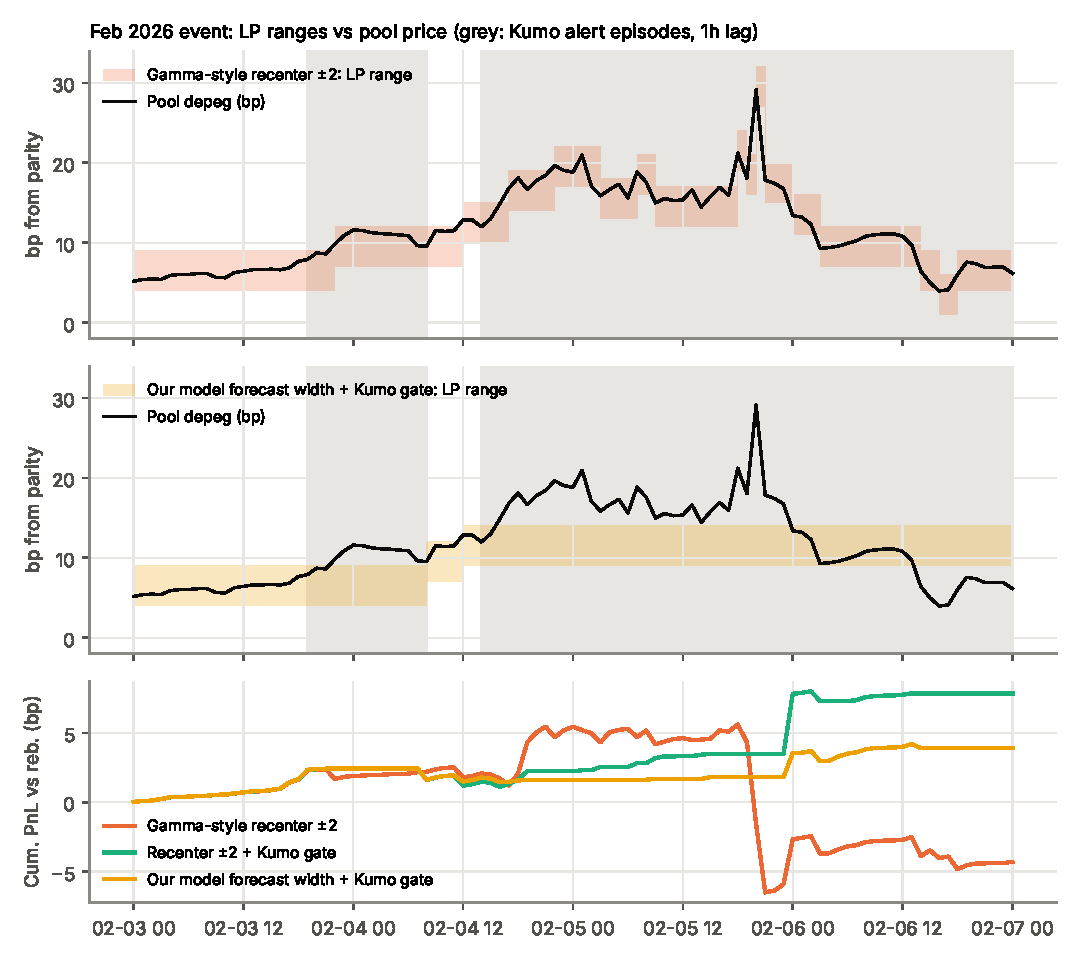
\includegraphics[width=\textwidth]{figures/lp_event_zoom.pdf}
    \caption{The February 2026 depeg. Top and middle: pool depeg (bp) and the range held by the
    ungated Gamma-style vault and by the two-model vault; grey areas are classifier alert
    episodes, shown with the one-hour execution lag. Bottom: cumulative net PnL against the
    rebalancing portfolio.\href{https://github.com/QuantLet/onchain-insights/tree/main/14.\%20LP\%20vault\%20backtest}{\includegraphics[height=0.6\baselineskip]{figures/Quantlet LOGO.png}}}
    \label{fig:lp_event}
\end{figure}

\subsubsection{Forecaster: range width and tail decisions}

The width rule rewards sharp predictive intervals as much as informative ones. TiDE earns the
most under the fixed rule (453\,bp per year) because its intervals are the narrowest: its
10\%--90\% interval covers the next hour 68\% of the time, against 95\% for our model, so its
vault holds tighter ranges and collects more fees in a calm year. To separate information from
width, Figure~\ref{fig:lp_width} scales each forecaster's half-width by a common factor and
compares net PnL at equal average width. At five ticks, our model, TiDE, TimeXer and GARCH earn
415--419\,bp per year, against 346\,bp for constant-width recentering. Any distributional
forecast thus adds 70--160\,bp per year below six ticks by widening ranges ahead of volatile
periods and narrowing them in calm ones, but range width does not discriminate between good
forecasters.

\begin{figure}[pos=!htbp,align=\centering]
    \centering
    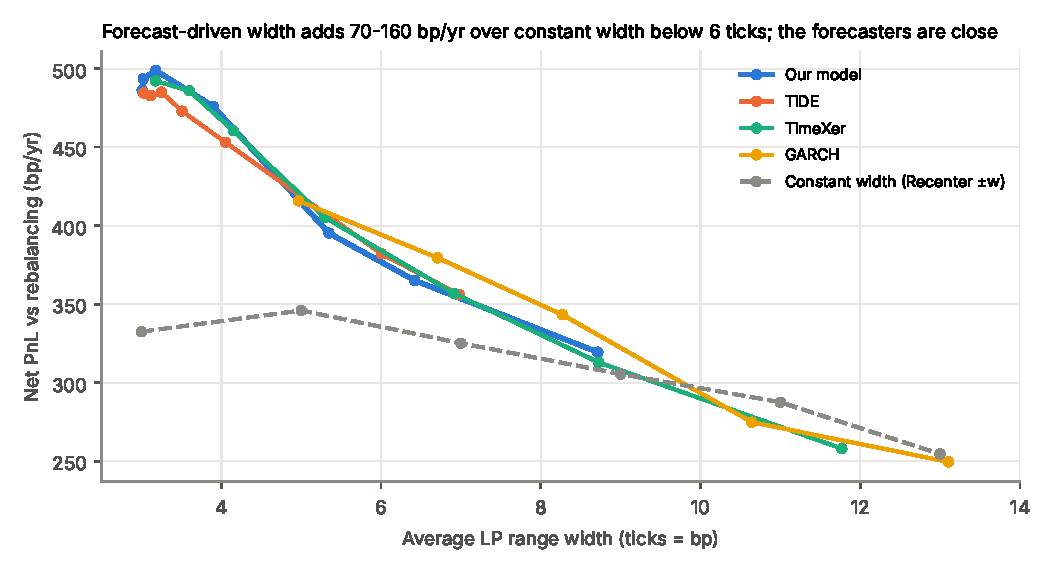
\includegraphics[width=0.85\textwidth]{figures/lp_width_frontier.pdf}
    \caption{Net PnL against average range width. Each forecaster's 10\%--90\% half-width is
    scaled by $k\in[0.25,2]$; the dashed line is constant-width recentering.\href{https://github.com/QuantLet/onchain-insights/tree/main/14.\%20LP\%20vault\%20backtest}{\includegraphics[height=0.6\baselineskip]{figures/Quantlet LOGO.png}}}
    \label{fig:lp_width}
\end{figure}

Tail decisions do discriminate (Table~\ref{tab:tail_value}). For exceedances of 10 and 15\,bp
at horizons of 6, 12 and 24 hours, our model obtains the best log score in five of six cases
and the lowest average Brier score. In the cost--loss problem it attains the highest relative
economic value in 8 of 18 threshold, horizon and cost settings, more than any benchmark. Its
advantage is largest in the extreme tail: at 15\,bp and 12 hours, with a cost--loss ratio of
0.2, its value is 0.27 against 0.11 for TiDE, while TimeXer ($-0.37$) and GARCH ($-1.00$) do
worse than the best constant policy. This is the decision-level counterpart of the
threshold-weighted CRPS results in Table~\ref{tab:benchmark}: TiDE and TimeXer produce sharp
central intervals, which pay in range setting, but less reliable tails, which are costly in
protection decisions.

\begin{table}[pos=!htbp,align=\centering]
\centering
\begin{threeparttable}
\caption{Tail-protection decisions from forecast exceedance probabilities
$\Pr(|d_{t+h}|\ge c)$, $c\in\{10,15\}$\,bp, $h\in\{6,12,24\}$ hours. Scores are averaged over
the six threshold--horizon cases. Value is the relative economic value $\mathcal V(r)$ of a
cost--loss protection rule; ``Top value'' counts the 18 threshold--horizon--cost settings
($r\in\{0.05,0.1,0.2\}$) in which the model attains the highest value.}
\label{tab:tail_value}
\small
\begin{tabular}{lrrrrr}
\toprule
Model & Log score & Brier & Top value & $\mathcal V(0.2)$ & $\mathcal V(0.2)$ \\
 & & & (of 18) & 15\,bp, 12h & 10\,bp, 24h \\
\midrule
Our model & \textbf{0.0460} & \textbf{0.0114} & \textbf{8} & \textbf{0.27} & \textbf{0.46} \\
Rolling empirical\tnote{a} & 0.0508 & 0.0132 & 7 & 0.05 & 0.40 \\
TiDE & 0.0560 & 0.0132 & 3 & 0.11 & 0.36 \\
TimeXer & 0.0564 & 0.0145 & 0 & $-0.37$ & 0.18 \\
GARCH & 0.0580 & 0.0141 & 0 & $-1.00$ & 0.38 \\
\bottomrule
\end{tabular}
\begin{tablenotes}\footnotesize
\item[a] Current depeg plus empirical quantiles of $h$-hour changes over the trailing 30 days.
\end{tablenotes}
\end{threeparttable}
\end{table}

\subsubsection{Tail-based strategies}

The forecaster's expected shortfall improves both the range and the gate. The ES band adds
24\,bp per year to the width rule for our model (95\% CI: 7--41, $p=0.002$) and lowers its
maximum drawdown from $-11.7$ to $-8.2$\,bp, because the range extends towards the heavier
tail instead of symmetrically. The ES-filtered gate keeps classifier alerts during 1.7\% of
hours instead of 11.6\%. It retains the drawdown reduction of the plain gate on both base vaults
while recovering most of its return cost: $+41$\,bp per year on the Gamma-style vault (CI:
15--75, $p=0.008$) and $+32$\,bp on the forecaster vault (CI: 5--67, $p=0.034$). Combining the
ES band with the ES-filtered gate gives the best risk-adjusted vault built on our model: 400\,bp
per year, Sharpe 15.0 and a maximum drawdown of $-2.5$\,bp, $+54$\,bp per year over the
two-model vault with the plain gate (CI: 22--93, $p=0.004$).

Two controls qualify these gains. Filtering classifier alerts by the current depeg instead of
the forecast, at the same alert share, performs similarly ($+7$\,bp per year in favour of the ES
filter, $p=0.26$), so much of the value comes from concentrating alerts in stressed conditions,
which the price level also reveals. Against random subsets of classifier episodes with the same
alert share, the ES filter improves the Sharpe ratio ($p=0.017$) but not significantly the
drawdown ($p=0.15$), since a single episode determines the drawdown. Across forecasters, the
combined rule ranks TiDE (447\,bp per year), the rolling-empirical benchmark (410) and our model
(400) ahead of TimeXer (322) and GARCH (263; Table~\ref{tab:lp_es}). Our model has the smallest
drawdown of the three leading vaults and outperforms TimeXer by 78\,bp per year (CI: 48--111).
Its difference to the rolling-empirical benchmark is not significant, and TiDE remains ahead.
Two tail rules do not pay: scaling deployed capital by the forecast ES lowers net PnL for every
forecaster, because resizing multiplies repositioning costs and idle capital earns nothing; and
holding an ES-wide range through classifier episodes performs no better than freezing.

\begin{table}[pos=!htbp,align=\centering]
\centering
\caption{Tail-based vault strategies across forecasters. ES band: asymmetric range from the
5\% expected shortfall over six hours, $\kappa=0.5$. ES-filtered gate: classifier alerts kept
only while the 24-hour ES lies more than 10\,bp from the current price; the alert share is the
fraction of hours frozen. Values in basis points of a \$1M vault.}
\label{tab:lp_es}
\resizebox{\textwidth}{!}{
\begin{tabular}{lrrrrrrr}
\toprule
 & \multicolumn{3}{c}{ES band} & \multicolumn{4}{c}{ES band + ES-filtered classifier} \\
\cmidrule(lr){2-4}\cmidrule(lr){5-8}
Forecaster & Net (bp/yr) & Sharpe & Max DD (bp) & Net (bp/yr) & Sharpe & Max DD (bp) & Alert share \\
\midrule
Our model & 420 & 13.9 & $-8.2$ & 400 & 15.0 & $-2.5$ & 1.7\% \\
TimeXer & 342 & 11.3 & $-3.8$ & 322 & 12.6 & $-2.3$ & 8.0\% \\
TiDE & 451 & 14.7 & $-5.0$ & 447 & 15.8 & $-3.9$ & 2.2\% \\
GARCH & 284 & 14.3 & $-1.9$ & 263 & 15.0 & $-1.9$ & 10.0\% \\
Rolling empirical & 437 & 13.5 & $-8.1$ & 410 & 15.7 & $-3.4$ & 2.4\% \\
\bottomrule
\end{tabular}
}
\end{table}

\subsubsection{Robustness and limitations}

The ranking of strategies is robust to gas and slippage costs, vault size, the execution lag
and fee reinvestment (Table~\ref{tab:lp_sensitivity}). Reinvesting accrued fees at each
repositioning, as automated vaults do, adds up to 17\,bp per year and leaves every comparison
unchanged. Absolute levels are sensitive to the share of fees captured by just-in-time
liquidity, which hourly snapshots of active liquidity exclude: if half of the fees accrue to
such liquidity, the forecaster vault still earns 65\,bp per year and the Gamma-style vault
loses 13\,bp. Four limitations apply. The evaluation covers one pool and five events; hourly
discretisation understates LVR and ignores intra-hour execution risk; a \$1M vault holds
about a tenth of in-range liquidity when its range is narrow; and every forecaster's largest
drawdown stems from a single four-hour spike to 29\,bp on 5 February 2026.


% -------------------------------------------------------------------------------------
% [F] CONCLUSION -- insert as a new paragraph after the second paragraph of Sec. 5
% -------------------------------------------------------------------------------------
The economic evaluation shows how the two models create value in different decisions. In a
liquidity-provision vault on the monitored pool, ranges set from the forecaster's quantiles
earn 395 basis points per year net of loss-versus-rebalancing and costs, significantly more
than Gamma-style and volatility-scaled benchmarks. At matched range width, however, the neural
forecasters perform similarly, because range setting rewards accurate central intervals. The
forecaster's distinctive contribution appears in tail-protection decisions, where its
exceedance probabilities obtain the best scores and the highest economic value in the most
settings. The classifier reduces the vault's drawdowns and daily tail losses significantly
relative to randomly timed alerts, but a contemporaneous price trigger achieves a similar
reduction for an LP that rebalances hourly. Using the forecaster's expected shortfall to shape
ranges and to filter alerts yields the best risk-adjusted vault on our model, 400 basis points
per year with a maximum drawdown of 2.5 basis points, although a well-calibrated empirical
tail benchmark and TiDE achieve comparable or higher returns under the same rules. Its lead time should be most valuable for decisions
that take time or become costlier as liquidity thins, such as unwinding large or leveraged
positions, which we leave for future work.


% -------------------------------------------------------------------------------------
% [G] APPENDIX -- new section, e.g. after "Probabilistic Forecasting Architecture"
% -------------------------------------------------------------------------------------
\section{Economic evaluation: supplementary results}\label{sec:econ_appendix}

\begin{table}[pos=!htbp,align=\centering]
\centering
\caption{All vault strategies, 15 January 2025 to 4 May 2026, in basis points of a \$1M vault.
Event windows sum net PnL from 24 hours before to 48 hours after each of the five events.
``Width'' rows use the 10\%--90\%, six-hour width rule. ``Tail range'' replaces the freeze by
the 1\%--99\% 24-hour interval during alert episodes. Sortino ratios are computed on hourly net
PnL; they are highest for wide, low-return ranges that rarely lose.}
\label{tab:lp_full}
\resizebox{\textwidth}{!}{
\begin{tabular}{lrrrrrrrrrr}
\toprule
Strategy & Fees & LVR & Costs & Net & Sharpe & Sortino & Max DD & Worst day & Reposit./month & Event windows \\
\midrule
Static $\pm5$ & 219 & $-44$ & 0 & 175 & 14.3 & 249.4 & $-0.5$ & $-0.1$ & 0.1 & 13 \\
Recenter $\pm2$ & 718 & $-186$ & $-186$ & 346 & 10.6 & 23.6 & $-12.1$ & $-11.1$ & 18.8 & 73 \\
Volatility-scaled & 457 & $-94$ & $-83$ & 281 & 10.8 & 32.7 & $-4.6$ & $-1.0$ & 9.2 & 74 \\
Recenter $\pm2$ + classifier freeze & 575 & $-131$ & $-135$ & 309 & 13.4 & 27.8 & $-4.5$ & $-1.5$ & 13.6 & 47 \\
Recenter $\pm2$ + classifier, parity $\pm15$ & 553 & $-115$ & $-155$ & 283 & 11.0 & 25.3 & $-4.5$ & $-3.0$ & 18.3 & 55 \\
Recenter $\pm2$ + ES-filtered classifier & 668 & $-162$ & $-157$ & 350 & 13.0 & 28.5 & $-4.5$ & $-2.4$ & 15.9 & 67 \\
Recenter $\pm2$ + price trigger & 558 & $-128$ & $-123$ & 307 & 14.1 & 28.9 & $-4.3$ & $-1.5$ & 12.4 & 21 \\
Recenter $\pm2$ + oracle & 631 & $-149$ & $-164$ & 317 & 12.9 & 25.6 & $-4.6$ & $-2.4$ & 16.5 & 34 \\
Our model width & 661 & $-160$ & $-106$ & 395 & 13.3 & 37.3 & $-11.7$ & $-1.1$ & 19.7 & 85 \\
Our model ES band & 713 & $-166$ & $-127$ & 420 & 13.9 & 42.1 & $-8.2$ & $-1.2$ & 22.4 & 88 \\
TimeXer width & 572 & $-128$ & $-88$ & 357 & 13.0 & 42.8 & $-6.5$ & $-1.2$ & 15.0 & 81 \\
TiDE width & 806 & $-193$ & $-159$ & 453 & 14.0 & 42.9 & $-7.4$ & $-2.2$ & 33.6 & 79 \\
GARCH width & 364 & $-75$ & $-39$ & 250 & 13.1 & 68.4 & $-1.7$ & $-0.7$ & 13.2 & 50 \\
ARIMA width & 150 & $-28$ & $-1$ & 121 & 6.4 & 79.7 & $-1.5$ & $-0.7$ & 0.2 & 57 \\
Naive width & 130 & $-23$ & $-1$ & 105 & 6.0 & 66.3 & $-2.2$ & $-0.8$ & 0.2 & 54 \\
Rolling empirical width & 692 & $-171$ & $-111$ & 410 & 12.6 & 34.9 & $-15.4$ & $-10.0$ & 21.9 & 74 \\
Our model width + classifier freeze & 550 & $-122$ & $-82$ & 346 & 14.7 & 49.5 & $-2.0$ & $-1.1$ & 14.2 & 42 \\
Our model width + classifier tail range & 565 & $-118$ & $-100$ & 346 & 13.8 & 48.0 & $-2.0$ & $-1.4$ & 18.6 & 62 \\
Our model width + ES-filtered classifier & 624 & $-144$ & $-100$ & 379 & 14.7 & 47.4 & $-2.8$ & $-1.1$ & 18.1 & 66 \\
Our model ES band + ES-filtered classifier & 678 & $-151$ & $-126$ & 400 & 15.0 & 45.9 & $-2.5$ & $-1.2$ & 21.6 & 66 \\
\bottomrule
\end{tabular}
}
\end{table}

\begin{table}[pos=!htbp,align=\centering]
\centering
\caption{Placebo test of classifier timing: 500 schedules placing the classifier's 43 alert
episodes, with their durations, at random dates under the same freeze rule. The $p$-value is
the share of placebo schedules performing at least as well as the classifier.}
\label{tab:lp_placebo}
\resizebox{\textwidth}{!}{
\begin{tabular}{llrrrr}
\toprule
Vault & Metric & Classifier & Placebo median & Placebo 5\%--95\% & $p$-value \\
\midrule
Recenter $\pm2$ & Net (bp/yr) & 309 & 343 & 326 -- 354 & 0.998 \\
 & Sharpe & 13.4 & 10.7 & 10.2 -- 11.5 & $<0.002$ \\
 & Max DD (bp) & $-4.5$ & $-12.1$ & $-12.2$ -- $-4.5$ & 0.020 \\
 & Worst day (bp) & $-1.5$ & $-11.1$ & $-11.2$ -- $-2.4$ & 0.008 \\
 & Daily CVaR 5\% (bp) & $-0.81$ & $-1.35$ & $-1.44$ -- $-0.92$ & 0.002 \\
\midrule
Our model width & Net (bp/yr) & 346 & 388 & 372 -- 398 & 1.000 \\
 & Sharpe & 14.7 & 13.1 & 12.7 -- 13.7 & 0.002 \\
 & Max DD (bp) & $-2.0$ & $-11.7$ & $-14.7$ -- $-2.8$ & 0.030 \\
 & Worst day (bp) & $-1.1$ & $-1.1$ & $-3.6$ -- $-0.8$ & 0.788 \\
\bottomrule
\end{tabular}
}
\end{table}

\begin{table}[pos=!htbp,align=\centering]
\centering
\caption{Differences in daily net PnL between the vault driven by our forecaster and
alternatives (10\%--90\%, six-hour width rule), annualised in basis points. Confidence
intervals from the stationary bootstrap with a mean block length of seven days (2,000 draws);
one-sided $p$-values test $H_0$: no improvement.}
\label{tab:lp_bootstrap}
\begin{tabular}{lrrr}
\toprule
Our model width versus & Difference (bp/yr) & 95\% CI & $p$-value \\
\midrule
Volatility-scaled & $+114$ & $[+73,\,+160]$ & $<0.001$ \\
Recenter $\pm2$ & $+49$ & $[+23,\,+80]$ & $<0.001$ \\
TimeXer width & $+38$ & $[+10,\,+68]$ & 0.007 \\
GARCH width & $+145$ & $[+102,\,+192]$ & $<0.001$ \\
ARIMA width & $+274$ & $[+220,\,+337]$ & $<0.001$ \\
Naive width & $+289$ & $[+231,\,+357]$ & $<0.001$ \\
TiDE width & $-58$ & $[-82,\,-34]$ & 1.000 \\
Rolling empirical width & $-15$ & $[-41,\,+16]$ & 0.86 \\
\bottomrule
\end{tabular}
\end{table}

\begin{table}[pos=!htbp,align=\centering]
\centering
\caption{Gating in 2024 (cross-validation test folds, 18 events). Classifier alerts are the
out-of-fold alert onsets of the selected specification; episode length is set to the holdout
median of 21 hours because hourly cross-validation scores were not retained.}
\label{tab:lp_2024}
\small
\begin{tabular}{lrrrr}
\toprule
Strategy & Net (bp/yr) & Sharpe & Max DD (bp) & Worst day (bp) \\
\midrule
Static $\pm5$ & 246 & 10.7 & $-28.4$ & $-3.6$ \\
Recenter $\pm2$ & 22 & 0.2 & $-455.6$ & $-45.4$ \\
\quad + classifier freeze & 182 & 2.3 & $-291.0$ & $-43.5$ \\
\quad + price trigger freeze & 271 & 5.7 & $-180.0$ & $-12.4$ \\
\quad + oracle freeze & 191 & 3.2 & $-278.0$ & $-12.6$ \\
Volatility-scaled & 253 & 6.9 & $-123.9$ & $-7.0$ \\
\quad + classifier freeze & 254 & 6.5 & $-121.9$ & $-14.1$ \\
\quad + price trigger freeze & 263 & 8.4 & $-93.7$ & $-5.7$ \\
\quad + oracle freeze & 261 & 7.9 & $-104.1$ & $-5.9$ \\
\bottomrule
\end{tabular}
\end{table}

\begin{table}[pos=!htbp,align=\centering]
\centering
\caption{Sensitivity of net PnL (bp per year; maximum drawdown in bp in parentheses).
``Fees reinvested'' adds accrued fees to the position at each repositioning; the threshold
variant also collects and reinvests whenever accrued fees exceed 0.1\% of capital. ``JIT
50\%'' assumes half of pool fees accrue to just-in-time liquidity.}
\label{tab:lp_sensitivity}
\resizebox{\textwidth}{!}{
\begin{tabular}{lrrrrr}
\toprule
Scenario & Recenter $\pm2$ & + classifier & + price trigger & Our model width & + classifier \\
\midrule
Base (\$1M, \$10 gas, 1.5\,bp swap) & 346 ($-12.1$) & 309 ($-4.5$) & 307 ($-4.3$) & 395 ($-11.7$) & 346 ($-2.0$) \\
Fees reinvested at repositioning & 357 ($-13.6$) & 318 ($-4.6$) & 316 ($-4.4$) & 408 ($-12.7$) & 357 ($-2.1$) \\
Fees reinvested, threshold & 357 ($-13.6$) & 317 ($-4.6$) & 315 ($-4.4$) & 407 ($-12.7$) & 355 ($-2.1$) \\
Low cost (\$2 gas, no slippage) & 420 ($-11.2$) & 362 ($-3.0$) & 356 ($-2.9$) & 442 ($-11.4$) & 382 ($-1.2$) \\
High cost (\$50 gas, 2\,bp swap) & 200 ($-21.3$) & 203 ($-13.0$) & 210 ($-9.8$) & 273 ($-13.3$) & 256 ($-6.9$) \\
\$100k vault & 338 ($-17.5$) & 258 ($-11.0$) & 251 ($-12.5$) & 349 ($-12.0$) & 285 ($-10.0$) \\
\$5M vault & 137 ($-26.3$) & 159 ($-8.9$) & 170 ($-4.7$) & 216 ($-12.3$) & 209 ($-5.0$) \\
JIT 50\% & $-13$ ($-35.5$) & 21 ($-15.8$) & 28 ($-17.4$) & 65 ($-13.2$) & 71 ($-7.0$) \\
\bottomrule
\end{tabular}
}
\end{table}
